% !TEX root = ../main.tex

\clearpage
% Source PDF page 10.
\section{第五章\quad 捧腹大笑思想理论体系}

捧腹大笑对年轻人有什么魔力？关于这个问题，我们可以通过深入的思考，建立奶蛙捧腹大笑思想理论体系（迫真）。~(见\figref{fig:05-1})

% !TEX root = ../../main.tex
\begin{figure}[H]
  \centering
  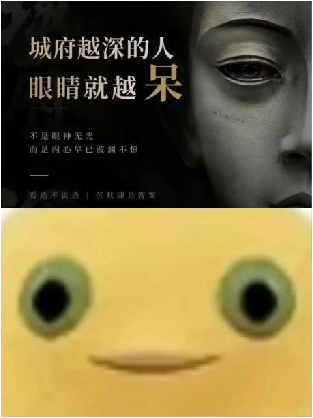
\includegraphics[width=127.74bp,height=0.76\textheight,keepaspectratio]{figures/chapter05/figure05_1.pdf}
  \renewcommand{\thefigure}{5.1}
  \caption{奶蛙的城府.jpg}
  \label{fig:05-1}
\end{figure}


\subsection{一、情绪代偿：把“绷不住”合法化}

考研、绩点、就业的复合压力下，负面情绪缺少体面的出口。奶蛙提供了一种\textquotedbl{}笑着崩溃\textquotedbl{}的姿态——既表达了失控，又不至于沉重。~(见\figref{fig:05-2})

% !TEX root = ../../main.tex
\begin{figure}[H]
  \centering
  
\includegraphics[width=128.76bp,height=0.76\textheight,keepaspectratio]{figures/chapter05/figure05_2.pdf}
  \renewcommand{\thefigure}{5.2}
  \caption{奶蛙的请假条}
  \label{fig:05-2}
\end{figure}


\subsection{二、群体稀释：用“我们”消解“我”}

用一张梗图代替自述，把“我很差劲”翻译成“我们都这样”。个体暴露被群体化收编，自嘲因而不必付出羞耻成本。~(见\figref{fig:05-3})

% !TEX root = ../../main.tex
\begin{figure}[H]
  \centering
  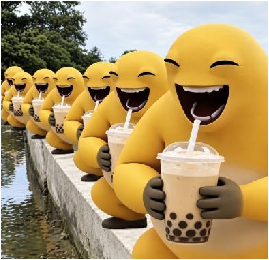
\includegraphics[width=109.89bp,height=0.76\textheight,keepaspectratio]{figures/chapter05/figure05_3.pdf}
  \renewcommand{\thefigure}{5.3}
  \caption{大家都在大笑，就不显得我糖了}
  \label{fig:05-3}
\end{figure}


\clearpage
% Source PDF page 11.
\subsection{三、反精致：对优秀人设的审美罢工}

大学生被期待为“精致的、上进的、有规划的人”。转发一只丑、怪、抽象的奶蛙，是一次低成本的不合作表态。~(见\figref{fig:05-4})

% !TEX root = ../../main.tex
\begin{figure}[H]
  \centering
  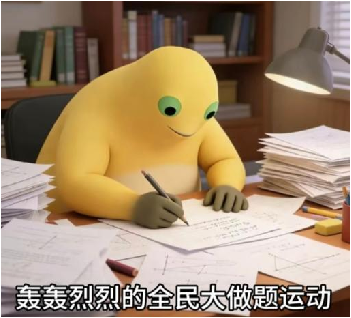
\includegraphics[width=143.14bp,height=0.76\textheight,keepaspectratio]{figures/chapter05/figure05_4.pdf}
  \renewcommand{\thefigure}{5.4}
  \caption{做题龙...？}
  \label{fig:05-4}
\end{figure}


\subsection{四、学校社交：人的本质是复读机}

集体居住让奶蛙拥有“线上”“面对面”双通道传播途径。同一个梗在同一屋檐下被反复复诵，趣味衰减极慢。~(见\figref{fig:05-5})

% !TEX root = ../../main.tex
\begin{figure}[H]
  \centering
  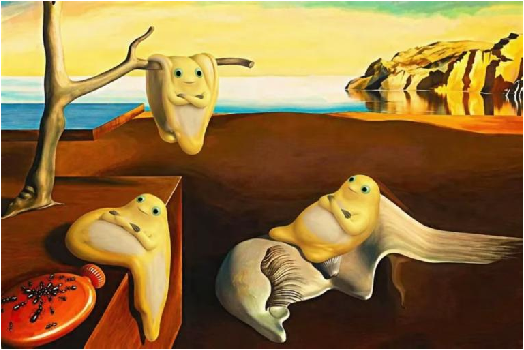
\includegraphics[width=213.93bp,height=0.76\textheight,keepaspectratio]{figures/chapter05/figure05_5.pdf}
  \renewcommand{\thefigure}{5.5}
  \caption{世界名画：永恒的奶蛙}
  \label{fig:05-5}
\end{figure}


\subsection{五、逆反认证：官方压制变成亚文化勋章}

2026 年 3 月，奶龙官方关评、拉黑，反而被网友读作“官方破防”。权威的否认，成了 meme 含金量的最高背书，热度此后一发不可收拾。~(见\figref{fig:05-6})

% !TEX root = ../../main.tex
\begin{figure}[H]
  \centering
  
\includegraphics[width=107.64bp,height=0.76\textheight,keepaspectratio]{figures/chapter05/figure05_6.pdf}
  \renewcommand{\thefigure}{5.6}
  \caption{喂，你打压奶蛙打压的很开心啊（全恼）}
  \label{fig:05-6}
\end{figure}


（不行，扯不下去了）

奶蛙：五重战神，出来！

如此的大笑魔神，又有谁能挡？！TM 的有谁能挡了？！

